\documentclass[12pt,a4paper]{article}
\usepackage[utf8]{inputenc}
\usepackage[margin=1in]{geometry}
\usepackage{graphicx}
\usepackage{hyperref}
\usepackage{xcolor}
\usepackage{tikz}
\usepackage{enumitem}
\usepackage{fontawesome5}
\usepackage{tcolorbox}
\usepackage{booktabs}
\usepackage{tabularx}
\usepackage{fancyhdr}
\usepackage{titlesec}

% Colors
\definecolor{primary}{RGB}{0, 0, 0}
\definecolor{accent}{RGB}{16, 185, 129}
\definecolor{lightgray}{RGB}{245, 245, 245}

% Header/Footer
\pagestyle{fancy}
\fancyhf{}
\fancyhead[L]{\textbf{iHire} - Hiring Intelligence System}
\fancyhead[R]{\thepage}
\fancyfoot[C]{\small Priyanshu | IIT Roorkee}

% Title formatting
\titleformat{\section}{\Large\bfseries\color{primary}}{}{0em}{}[\titlerule]
\titleformat{\subsection}{\large\bfseries\color{primary}}{}{0em}{}

% Hyperlink setup
\hypersetup{
    colorlinks=true,
    linkcolor=accent,
    urlcolor=accent,
}

\begin{document}

% Title Page
\begin{titlepage}
    \centering
    \vspace*{2cm}
    
    {\Huge\bfseries iHire}\\[0.5cm]
    {\Large Multi-Agent Hiring Intelligence System}\\[2cm]
    
    
\begin{tikzpicture}
        \draw[line width=2pt, accent] (0,0) circle (1.5cm);
        \node at (0,0) {\Huge\faUserTie};
    \end{tikzpicture}
    
    \vspace{2cm}
    
    {\large A Production-Ready, Enterprise-Grade Solution for\\Automated Resume Screening \& Candidate Evaluation}
    
    \vspace{3cm}
    
    \begin{tcolorbox}[colback=lightgray, colframe=primary, width=0.8\textwidth]
        \centering
        \textbf{Developed By}\\[0.3cm]
        {\Large Priyanshu}\\[0.2cm]
        B.Tech, IIT Roorkee\\[0.3cm]
        \faEnvelope\ \href{mailto:priyanshu@me.iitr.ac.in}{priyanshu@me.iitr.ac.in}\\[0.1cm]
        \faPhone\ +91 9821040290\\[0.1cm]
        \faGithub\ \href{https://github.com/i24hour/iHire}{github.com/i24hour/iHire}
    \end{tcolorbox}
    
    \vspace{0.8cm}
    
    \begin{tcolorbox}[colback=accent!10, colframe=accent, width=0.8\textwidth]
        \centering
        \textbf{Live Links}\\[0.3cm]
        \faGlobe\ Dashboard: \href{https://frontend-beta-six-90.vercel.app}{frontend-beta-six-90.vercel.app}\\[0.1cm]
        \faFolder\ Resume Folder: \href{https://drive.google.com/drive/folders/1atZ_Msur-JdjYKfqniLqBhYf9BxQthIk}{Google Drive}\\[0.1cm]
        \faTable\ Results Sheet: \href{https://docs.google.com/spreadsheets/d/1Y34ICh4tEfbVbD6cszBVj7JYO6tyWewfyXoJO2wtKTc}{Google Sheet}
    \end{tcolorbox}
    
    \vfill
\end{titlepage}

\tableofcontents
\newpage

% ============================================
\section{Quick Start Guide - How to Use}
% ============================================

\begin{tcolorbox}[colback=accent!5, colframe=accent, title=\textbf{Simple 3-Step Process}]
Using iHire is very simple. Just follow these three steps:
\end{tcolorbox}

\subsection{Step 1: Upload Resumes to Google Drive}

\begin{enumerate}
    \item Open the \textbf{Resume Folder}: \href{https://drive.google.com/drive/folders/1atZ_Msur-JdjYKfqniLqBhYf9BxQthIk}{Click Here}
    \item Create a \textbf{new folder} for each job role (e.g., ``Frontend Developer'', ``Product Manager'')
    \item Inside each folder, upload:
    \begin{itemize}
        \item One \textbf{Job Description PDF} (filename should contain ``JD'' or ``Job'')
        \item All \textbf{candidate resume PDFs}
    \end{itemize}
\end{enumerate}

\textbf{That's it!} The system automatically detects new files every 30 seconds.

\subsection{Step 2: View Results in Dashboard}

\begin{enumerate}
    \item Open the \textbf{Dashboard}: \href{https://frontend-beta-six-90.vercel.app}{Click Here}
    \item Select your job role from the \textbf{sidebar} on the left
    \item View all candidates with their:
    \begin{itemize}
        \item \textbf{Relevance Score} (0-100) - Overall fit for the role
        \item \textbf{Recommendation} - Strong Yes / Yes / Maybe / Not Now
        \item \textbf{Assignment Brief} - Role-specific task for the candidate
    \end{itemize}
\end{enumerate}

\subsection{Step 3: Check Detailed Data in Google Sheet}

\begin{enumerate}
    \item Open the \textbf{Results Sheet}: \href{https://docs.google.com/spreadsheets/d/1Y34ICh4tEfbVbD6cszBVj7JYO6tyWewfyXoJO2wtKTc}{Click Here}
    \item Each job role has its own \textbf{tab} at the bottom
    \item View detailed scores, feedback, and assignment for each candidate
\end{enumerate}

\begin{tcolorbox}[colback=yellow!10, colframe=orange, title=\textbf{Important Note}]
The system processes resumes automatically in the background. After uploading, wait 2-3 minutes for results to appear in the dashboard and sheet.
\end{tcolorbox}

\newpage

% ============================================
\section{Executive Summary}
% ============================================

In today's competitive job market, hiring managers spend an average of 23 hours screening resumes for a single position. With hundreds of applications per role, this process is not only time-consuming but also prone to human bias and inconsistency. \textbf{iHire} addresses these challenges head-on.

iHire is an \textbf{industry-scale, multi-agent AI system} designed to automate and enhance the hiring process. Unlike basic keyword-matching tools, iHire employs a sophisticated pipeline of specialized AI agents that analyze resumes with the same rigor a founding team would apply when building their core team.

\subsection{Key Value Propositions}

\begin{itemize}[leftmargin=*]
    \item \textbf{80\% Reduction in Screening Time} - Automated processing within minutes of resume upload
    \item \textbf{Consistent Evaluation Criteria} - Same rigorous standards applied to every candidate
    \item \textbf{Multi-Campaign Support} - Handle multiple job roles simultaneously
    \item \textbf{Role-Specific Assignments} - Auto-generated technical assessments per JD
    \item \textbf{Real-time Dashboard} - Live tracking with actionable insights
\end{itemize}

% ============================================
\section{Problem Statement}
% ============================================

Traditional hiring faces several critical challenges:

\begin{enumerate}
    \item \textbf{Volume Overload}: A single job posting can attract 200-500 applications
    \item \textbf{Inconsistent Screening}: Different reviewers apply different criteria
    \item \textbf{Time Constraints}: HR teams often rush through resumes, missing quality candidates
    \item \textbf{Bias Introduction}: Unconscious biases affect decision-making
    \item \textbf{Generic Assessments}: One-size-fits-all assignments don't test role-specific skills
\end{enumerate}

\begin{tcolorbox}[colback=lightgray, colframe=accent, title=\textbf{The iHire Solution}]
A systematic, AI-powered approach that combines multiple specialized agents to evaluate candidates from different perspectives - technical fit, founder confidence, and role-specific compatibility - producing consistent, explainable, and actionable recommendations.
\end{tcolorbox}

% ============================================
\section{System Architecture}
% ============================================

iHire follows a \textbf{microservices-inspired architecture} with clear separation of concerns:

\subsection{High-Level Architecture}

\begin{center}
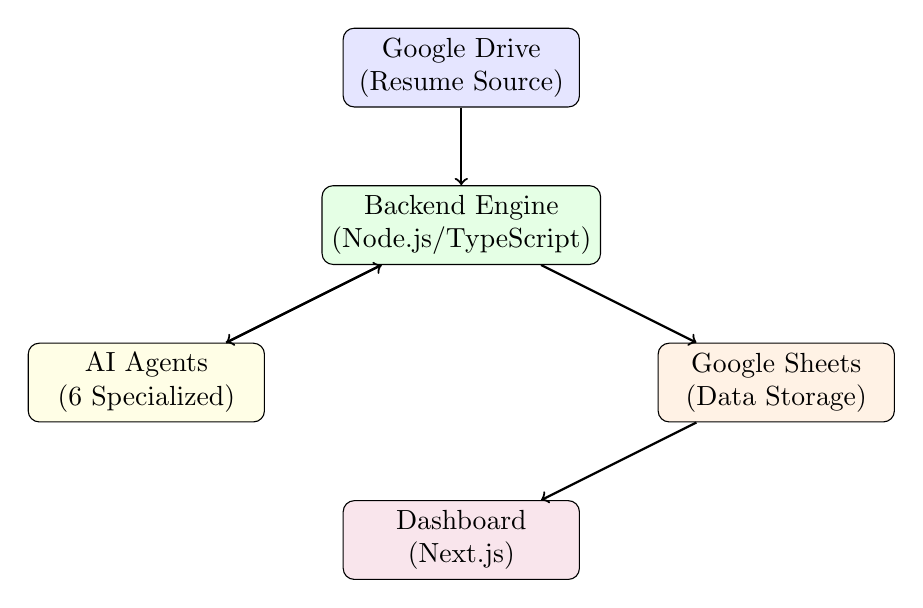
\begin{tikzpicture}[
    box/.style={draw, rounded corners, minimum width=3cm, minimum height=1cm, align=center},
    arrow/.style={->, thick}
]
    % Google Drive
    \node[box, fill=blue!10] (drive) at (0,4) {Google Drive\\(Resume Source)};
    
    % Backend
    \node[box, fill=green!10] (backend) at (0,2) {Backend Engine\\(Node.js/TypeScript)};
    
    % Agents
    \node[box, fill=yellow!10] (agents) at (-4,0) {AI Agents\\(6 Specialized)};
    
    % Google Sheets
    \node[box, fill=orange!10] (sheets) at (4,0) {Google Sheets\\(Data Storage)};
    
    % Frontend
    \node[box, fill=purple!10] (frontend) at (0,-2) {Dashboard\\(Next.js)};
    
    % Arrows
    \draw[arrow] (drive) -- (backend);
    \draw[arrow] (backend) -- (agents);
    \draw[arrow] (backend) -- (sheets);
    \draw[arrow] (sheets) -- (frontend);
    \draw[arrow] (agents) -- (backend);
\end{tikzpicture}
\end{center}

\subsection{Component Breakdown}

\begin{table}[h]
\centering
\begin{tabularx}{\textwidth}{lX}
\toprule
\textbf{Component} & \textbf{Responsibility} \\
\midrule
Drive Monitor & Watches for new resumes, detects campaign folders \\
Workflow Orchestrator & Coordinates agent pipeline, manages state \\
AI Agent Pipeline & Six specialized agents for comprehensive analysis \\
Sheets Writer & Persists results, manages campaign-specific tabs \\
Email Notifier & Sends assignments to qualified candidates \\
Frontend Dashboard & Real-time visualization and campaign management \\
\bottomrule
\end{tabularx}
\end{table}

% ============================================
\section{Multi-Agent Pipeline}
% ============================================

The core innovation of iHire lies in its \textbf{multi-agent architecture}. Rather than using a single AI model, we employ six specialized agents, each focused on a specific aspect of candidate evaluation.

\subsection{Agent 1: JD Reality Agent}

\textbf{Purpose}: Analyze the Job Description to extract structured requirements.

\textbf{Outputs}:
\begin{itemize}
    \item Core work responsibilities
    \item Non-negotiable skills
    \item Role context (Startup Execution, High Ownership, etc.)
    \item Ownership \& pressure levels
    \item Criticality factor (C $\in$ [0.6, 1.0])
\end{itemize}

\subsection{Agent 2: Resume Structuring Agent}

\textbf{Purpose}: Parse unstructured resume PDFs into structured candidate profiles.

\textbf{Outputs}:
\begin{itemize}
    \item Work experience with achievements
    \item Skills with confidence levels
    \item Projects with impact metrics
    \item Education background
\end{itemize}

\subsection{Agent 3: Technical Checking Agent}

\textbf{Purpose}: Evaluate technical fit using the \textbf{Execution Fit Score} formula:

\begin{equation}
E = 100 \times (w_S \cdot S + w_D \cdot D + w_W \cdot W - w_R \cdot R)
\end{equation}

Where:
\begin{itemize}
    \item $S$ = Skill relevance (0-1)
    \item $D$ = Depth of evidence (0-1)
    \item $W$ = Work similarity (0-1)
    \item $R$ = Risk penalty (0-1)
\end{itemize}

\subsection{Agent 4: Founder Confidence Agent}

\textbf{Purpose}: Evaluate soft factors a founder would consider.

\textbf{Formula} (role-context weighted):
\begin{equation}
F = 100 \times (w_O \cdot O + w_L \cdot L + w_P \cdot P + w_G \cdot G)
\end{equation}

Where weights $(w_O, w_L, w_P, w_G)$ vary by role context:
\begin{itemize}
    \item \textbf{Early Startup}: High ownership (0.35), high pressure handling (0.30)
    \item \textbf{Stable Long-Term}: High longevity (0.40), high growth (0.25)
\end{itemize}

\subsection{Agent 5: Relevance Synthesizer}

\textbf{Purpose}: Combine scores into a final relevance score.

\begin{equation}
R = C \times (\alpha \cdot E + \beta \cdot F)
\end{equation}

Where $C$ is the criticality factor and $\alpha, \beta$ are role-specific weights.

\subsection{Agent 6: Assignment Generation Agent}

\textbf{Purpose}: Create role-specific, practical assignments.

\textbf{Key Feature}: One assignment per JD (not per candidate) - ensuring consistency in evaluation.

% ============================================
\section{Multi-Campaign Support}
% ============================================

iHire supports \textbf{multiple simultaneous hiring campaigns}, enabling organizations to manage several job roles in parallel.

\subsection{Folder Structure}

\begin{verbatim}
iHire_Campaigns/ (Root Folder)
|-- Senior_Frontend_Dev/
|   |-- JD.pdf
|   |-- candidate_1.pdf
|   +-- candidate_2.pdf
|-- Product_Manager/
|   |-- PM_JD.pdf
|   +-- applicant_resume.pdf
+-- Data_Scientist/
    |-- DS_Job_Description.pdf
    +-- resume.pdf
\end{verbatim}

\subsection{Automatic Detection}

\begin{itemize}
    \item System monitors root folder for new subfolders
    \item Each subfolder = One hiring campaign
    \item JD identified by filename containing "JD" or "Job"
    \item All other PDFs = Candidate resumes
\end{itemize}

\subsection{Isolated Processing}

\begin{itemize}
    \item Separate Google Sheet tab per campaign
    \item Campaign-specific relevance thresholds
    \item Independent assignment generation per JD
\end{itemize}

% ============================================
\section{Technical Stack}
% ============================================

\begin{table}[h]
\centering
\begin{tabularx}{\textwidth}{lXl}
\toprule
\textbf{Layer} & \textbf{Technology} & \textbf{Purpose} \\
\midrule
\multicolumn{3}{l}{\textbf{Backend}} \\
Runtime & Node.js 20+ & Server-side JavaScript \\
Language & TypeScript & Type-safe development \\
AI Integration & LiteLLM & Multi-provider AI abstraction \\
AI Models & Gemini 2.0 Flash & Fast, accurate inference \\
PDF Processing & pdf-parse & Resume text extraction \\
\midrule
\multicolumn{3}{l}{\textbf{Frontend}} \\
Framework & Next.js 14 & React with App Router \\
Styling & Tailwind CSS & Utility-first CSS \\
Animations & Framer Motion & Smooth UI transitions \\
\midrule
\multicolumn{3}{l}{\textbf{Infrastructure}} \\
Backend Hosting & Railway & Auto-scaling containers \\
Frontend Hosting & Vercel & Edge deployment \\
Storage & Google Sheets & Structured data persistence \\
File Source & Google Drive & Resume ingestion \\
Email & Gmail SMTP & Candidate notifications \\
\bottomrule
\end{tabularx}
\end{table}

% ============================================
\section{Frontend Dashboard}
% ============================================

The dashboard provides a \textbf{real-time, intuitive interface} for hiring teams.

\subsection{Key Features}

\begin{enumerate}
    \item \textbf{Campaign Switcher}: Sidebar shows all active jobs; click to filter
    \item \textbf{Candidate Table}: Sortable by relevance, execution fit, or date
    \item \textbf{Recommendation Badges}: Visual indicators (Strong Yes, Yes, Maybe, Not Now)
    \item \textbf{One-Click Assignment}: Send technical assignments directly from dashboard
    \item \textbf{Resume Viewer}: Quick access to original resume
    \item \textbf{Dark Theme}: Modern, professional interface
\end{enumerate}

\subsection{Scoring Visualization}

Each candidate displays:
\begin{itemize}
    \item \textbf{Relevance Score} (0-100): Overall fit
    \item \textbf{Execution Fit} (0-100): Technical capability
    \item \textbf{Founder Confidence} (0-100): Soft factors
\end{itemize}

% ============================================
\section{Email Integration}
% ============================================

Qualified candidates automatically receive personalized assignment emails:

\begin{tcolorbox}[colback=lightgray, colframe=primary]
\textbf{Subject}: Technical Assignment - [Role Name]\\[0.3cm]
Dear [Candidate Name],\\[0.2cm]
Congratulations on progressing to the next stage! We were impressed with your profile and would like you to complete a technical assessment.\\[0.3cm]
\textbf{Assignment}: [Role-Specific Task]\\
\textbf{Time Limit}: 4-6 hours\\
\textbf{Submission}: [Instructions]
\end{tcolorbox}

% ============================================
\section{Production Readiness}
% ============================================

iHire is designed for \textbf{enterprise deployment}:

\subsection{Scalability}
\begin{itemize}
    \item Stateless backend enables horizontal scaling
    \item Async processing prevents bottlenecks
    \item Campaign isolation allows parallel workloads
\end{itemize}

\subsection{Reliability}
\begin{itemize}
    \item Duplicate detection prevents re-processing
    \item Error handling with graceful degradation
    \item Persistent caching for JD analysis
\end{itemize}

\subsection{Security}
\begin{itemize}
    \item Service Account authentication for GCP
    \item Environment-based configuration
    \item No sensitive data in version control
\end{itemize}

\subsection{Extensibility}
\begin{itemize}
    \item Modular agent architecture
    \item Easy integration with ATS systems
    \item Support for multiple AI providers
\end{itemize}

% ============================================
\section{Use Cases}
% ============================================

\subsection{Startups}
Fast-moving teams can process hundreds of applications for multiple roles simultaneously, focusing founder time on final interviews only.

\subsection{HR Agencies}
Agencies managing hiring for multiple clients can create separate campaigns per client, ensuring isolated and consistent evaluation.

\subsection{Enterprise HR}
Large organizations can standardize their screening process across departments while maintaining role-specific customization.

% ============================================
\section{Future Roadmap}
% ============================================

\begin{enumerate}
    \item \textbf{ATS Integration}: Direct sync with Greenhouse, Lever, Workday
    \item \textbf{Video Interview Analysis}: AI-powered interview assessment
    \item \textbf{Bias Detection Module}: Identify and flag potential biases
    \item \textbf{Candidate Portal}: Self-service portal for applicants
    \item \textbf{Analytics Dashboard}: Hiring funnel metrics and insights
\end{enumerate}

% ============================================
\section{Conclusion}
% ============================================

iHire represents a paradigm shift in how organizations approach hiring. By combining the speed and consistency of AI with the nuanced evaluation criteria of experienced founders, it delivers a solution that is both efficient and effective.

The multi-agent architecture ensures that no single point of failure or bias can dominate the decision-making process. Each agent brings a unique perspective, and the synthesized result reflects a holistic view of candidate fit.

Whether you're a startup looking to build your founding team or an enterprise scaling your hiring operations, iHire provides the infrastructure to make informed, consistent, and timely hiring decisions.

\vspace{1cm}
\begin{center}
\begin{tcolorbox}[colback=accent!10, colframe=accent, width=0.8\textwidth]
\centering
\textbf{For any feedback feel free to contact us}\\[0.3cm]
Contact: \href{mailto:priyanshu@me.iitr.ac.in}{priyanshu@me.iitr.ac.in}\\
Phone: +91 9821040290\\
GitHub: \href{https://github.com/i24hour/iHire}{github.com/i24hour/iHire}
\end{tcolorbox}
\end{center}

\end{document}
